%%%%%%%%%%%%%%%%%%%%%%%%%%%%%%%%%%%%%%%%%%%%%%%%%%%%%%%%%%%%%%%%%
%%% %
%%% % weiiszablon.tex
%%% % The Faculty of Electrical and Computer Engineering
%%% % Rzeszow University Of Technology diploma thesis Template
%%% % Szablon pracy dyplomowej Wydziału Elektrotechniki 
%%% % i Informatyki PRz
%%% % June, 2015
%%%%%%%%%%%%%%%%%%%%%%%%%%%%%%%%%%%%%%%%%%%%%%%%%%%%%%%%%%%%%%%%%

\documentclass[12pt,twoside]{article}

\usepackage{weiiszablon}
\usepackage{csquotes}
\usepackage{float}
\usepackage{hyperref}

\author{Łukasz Miłoś}

% np. EF-123456, EN-654321, ...
\studentID{EF-161883}

\title{System zarządzania bazą BOM}

%%% wybierz rodzaj pracy wpisując jeden z poniższych numerów: ...
% 1 = inżynierska	% BSc
% 2 = magisterska	% MSc
% 3 = doktorska		% PhD
%%% na miejsce zera w linijce poniżej
\newcommand{\rodzajPracyNo}{0}

%%% promotor
\supervisor{(dr inż.) Mariusz Borkowski (prof. PRz)}
%% przykład: dr hab. inż. Józef Nowak, prof. PRz

%%% promotor ze stopniami naukowymi po angielsku
\supervisorEN{(EngD) Mariusz Borkowski}

\begin{document}

% strona tytułowa
\maketitle
\blankpage

% spis treści
\tableofcontents
\clearpage
\blankpage

\section{Wstęp}
Projekt dotyczy przedmiotu \enquote{Usługi sieciowe w biznesie} i zgodnie z założeniami ma ściśle praktyczny charakter.

Sam przedmiot skupia się na zagadnieniach informatyzacji w przedsiębiorstwach, które wpływają na ich organizację i strukturę. Dzięki zastosowaniu różnej klasy systemów, działania ludzkie są wspierane, a często także zastępowane poprzez wykorzystanie nowych technologii, co ma swoje odzwierciedlenie w większej wydajności, produktywności, mniejszym ryzyku popełnienia błędu, a co za tym idzie także minimalizacji kosztów operacyjnych. Wiele zagadnień w przedsiębiorstwach można ułatwić poprzez zastosowanie odpowiedniego systemu zintegrowanego, stąd niezbędna wiedza o typach, funkcjach i przypadkach użycia poszczególnych technologii.

Spośród mnogości zagadnień wybrano temat dotyczący organizacji zasobów produkcyjnych, jako bardzo istotny element wielu przedsiębiorstw.

W ramach projektu utworzono system zarządzania bazą BOM (Bill of Materials). Zagadnienie to jest ściśle związane z przedmiotem i zostanie opisane w kolejnym rozdziale.

\clearpage

\section{Opis problemu}

BOM (Bill Of Materials) jest strukturalnym (hierarchicznym) zestawieniem materiałowym produktu końcowego zawierającym listę części składowych niezbędnych do jego wytworzenia wraz z podaniem cech określających dany zasób m.in. ceny i ilości. Takie zestawienia są wykorzystywane na różnych etapach produkcji, zarówno podczas projektowania, a także podczas wytwarzania czy nawet montażu.

Niekiedy BOM jest wzbogacany o opis kolejnych czynności, w których używane są poszczególne elementy składowe (przykładem jest dowolna instrukcja szafy przeznaczonej do samodzielnego montażu, która często zawiera elementy składowe wraz z wyszczególnieniem kolejnych czynności montażowych).

Poszczególne elementy posiadają kilka cech (atrybutów). W zależności od implementacji systemu parametry są różne. Oto kilka najpopularniejszych z nich:

\begin{itemize}[label=-,labelsep=0.4cm,leftmargin=0.6cm]
\item identyfikator
\item nazwa
\item ilość
\item jednostka miary
\item cena jednostkowa
\item cena sumaryczna
\end{itemize}

Wyjściowym etapem w konstrukcji zestawienia materiałowego może być ogólne, koncepcyjne przedstawienie części składowych produktu finalnego w formie rysunku (\ref{fig:example:drawing}) lub grafu (\ref{fig:example:graph}).

\begin{figure}[h]
	\centering
	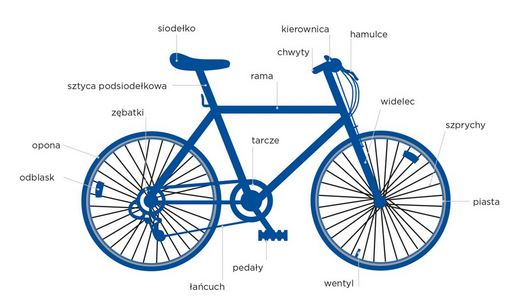
\includegraphics[width=\textwidth]{figures/examples/drawing.jpg}
	\caption{Przykład koncepcyjnego zestawienia BOM w formie rysunku [https://www.mecalux.pl/blog/zestawienie-materialowe-bom]}
\label{fig:example:drawing}
\end{figure}

Należy zwrócić uwagę, że poszczególne elementy składowe, także składają się z mniejszych komponentów (hierarchia). Ważne jest zaprezentowanie odpowiedniego stopnia złożoności, który zależy od specyfiki danego przedsiębiorstwa. Przykładowo dla firmy produkującej rowery, schemat (\ref{fig:example:drawing}) może okazać się wystarczający, jeśli korzysta ona z gotowych produktów innych firm, a nie tworzy wszystkiego na własną rękę. Przykładem jest tutaj półprodukt hamulca. O ile firma zakupuje gotowe hamulce od innej marki i tylko montuje je w swoich rowerach to ten poziom wyszczególnienia jest wystarczający. Natomiast w przypadku produkcji hamulców na wewnętrznie, należałoby dodatkowo wyszczególnić części składowe hamulca (m.in. rączkę, mocowanie, śruby mocujące, linkę, gumki ścieralne, gumki ochronne, smar itd.).

Innym sposobem koncepcyjnego zapisu zestawienia materiałowego dowolnego produktu może być graf (\ref{fig:example:graph}). Na podstawie grafu można przedstawić hierarchię, ale nie jest możliwe przedstawienie informacji szczegółowych dotyczących poszczególnych wyrobów.

\begin{figure}[h]
	\centering
	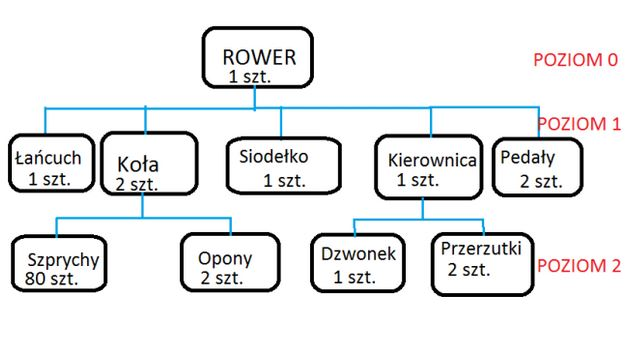
\includegraphics[width=\textwidth]{figures/examples/graph.jpg}
	\caption{Przykład koncepcyjnego zestawienia BOM w formie grafu [https://logistykanalogike.wordpress.com/2014/12/18/struktura-wyrobu/]}
\label{fig:example:graph}
\end{figure}

W rzeczywistości zestawienia materiałowe przyjmują jednak formę tabeli (\ref{fig:example:table}) lub hierarchii (\ref{fig:example:hierarchy}), z wyszczególnieniem poszczególnych elementów składowych.

\begin{figure}[h]
	\centering
	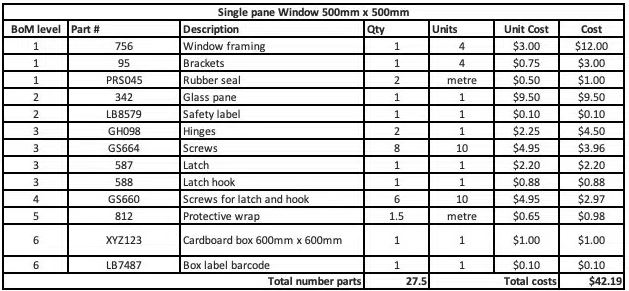
\includegraphics[width=\textwidth]{figures/examples/table.jpg}
	\caption{Przykład zestawienia BOM w formie tabeli [https://www.unleashedsoftware.com/blog/everything-you-need-to-know-about-bill-of-materials]}
\label{fig:example:table}
\end{figure}

Niestety wykorzystanie tabeli nie przedstawia wprost hierarchii poszczególnych komponentów. Hierarchia jest tutaj (\ref{fig:example:table}) oznaczona za pomocą pierwszej kolumny (BoM level). Zestawienie w formie tabeli w tym przypadku zawiera identyfikator części, opis, ilość, jednostkę, koszt jednostkowy i koszt całościowy.

Najlepszym sposobem prezentacji zestawienia materiałowego (BOM) jest pokazanie hierarchii (\ref{fig:example:hierarchy}), np. za pomocą drzewa hierachicznego (treeview).

\begin{figure}[h]
	\centering
	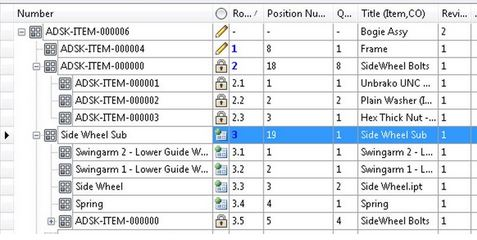
\includegraphics[width=\textwidth]{figures/examples/hierarchy.jpg}
	\caption{Przykład zestawienia BOM w formie drzewa hierarchicznego [https://underthehood-autodesk.typepad.com/blog/items/page/2/]}
\label{fig:example:hierarchy}
\end{figure}

Na załączonym zdjęciu (\ref{fig:example:hierarchy}) pokazano przykład docelowej hierarchii. Jest także możliwość rozwijania i zwijania poszczególnych elementów składowych, co pozwala zwiększyć czytelność zestawienia.

Temat organizacji zasobów produkcyjnych jest bardzo istotny, ponieważ umożliwia zachowanie ciągłości produkcji, a także pozwala na utrzymanie płynności finansowej przedsiębiorstwa.

Dzięki posiadaniu precyzyjnych zestawień można planować zakup surowców (ustrzeżenie się braku, ale także nadmiaru zapasów), a także określać niezbędne do poniesienia koszty (planowanie budżetu). Nie można również zapomnieć o tym, że mając wiedzę na temat niezbędnych materiałów i ich ilości można zarządzać zapasami na przyszłość i nie dopuścić do braku materiałów w magazynie, co jest bardzo niebezpieczne. Istotny jest także atut minimalizacji błędów, zyskany dzięki korzystaniu z utworzonego zestawienia.

Projekt jest zatem próbą znalezienia rozwiązania poprzez utworzenie własnego systemu do zarządzania hierarchiczną bazą BOM. Naturalnie takie systemy istnieją na rynku, ale są one zazwyczaj częścią zintegrowanych systemów zarządzania przedsiębiorstwem i nie stanowią oddzielnych bytów.

\clearpage
\section{Rozwiązanie}

Sekcję rozwiązania podzielono na 3 części: zalecenia, założenia i opis. Pierwsza z nich ogólnie przedstawia wyobrażenie idealnego systemu. Założenia są efektem podjęcia decyzji odnośnie wyboru technologii, która umożliwi realizację celu. Ostatnia z części stanowi opis systemu.

\subsection*{Zalecenia}
Analiza problemu doprowadziła do powstania pewnych zaleceń implementowanego systemu. Celem jest wykorzystanie zalet innych systemów, a także eliminacja ich wad. Najważniejsze zalecenia spisano poniżej:

\begin{itemize}[label=-,labelsep=0.4cm,leftmargin=0.6cm]
\item system ma być prosty i niezależny od innego oprogramowania (samodzielny)
\item bardzo istotna jest prezentacja zestawienia materiałowego w postaci hierarchii, a także pokazanie szczegółów poszczególnych wyrobów. 
\item program powinien posiadać wygodny i intuicyjny interfejs użytkownika
\item możliwość dodawania, usuwania i edycji poszczególnych pozycji zestawienia
\end{itemize}

\subsection*{Założenia}
Na podstawie założeń zdecydowano się na implementację systemu przy użyciu języka programowania Python i wbudowanej biblioteki do obsługi interfejsu graficznego o nazwie tkinter. Python został wybrany jako  przyszłościowy język wysokiego poziomu o wielorakich zastosowaniach. Biblioteka graficzna ułatwia proces tworzenia interfejsu graficznego i pozwala się skupić na faktycznej realizacji. Przy pomocy tych dwóch narzędzi można zorganizować niemal cały wymagany system.

Istotnym zagadnieniem jest jednak przechowywanie danych, ponieważ bez tego zestawienie istniałoby tylko podczas działania programu (przechowywane w pamięci). W celu uzyskania pełnej niezależności postawiono na przechowywanie zestawień w lokalnych plikach komputera w formacie JSON. Jest to tekstowy format zapisu danych, który już sam w sobie jest hierarchiczny.

Ważna jest także walidacja danych wejściowych (plików i interaktywnych pól tekstowych), a także obsługa błędów.

\subsection*{Opis}
Zgodnie z założeniami zrealizowano system przy użyciu wybranych technologii. Warto zwrócić uwagę na samodzielność realizacji poszczególnych zagadnień, a także samą stylistkę kodu, wykorzystującą programowanie zorientowane obiektowo.

W aplikacji zadbano o minimalistyczny, modernistyczny, responsywny interfejs użytkownika, a także obsługę wszelkich błędów.

Aplikacja składa się z kilku stron i wielu okien modalnych, wyświetlanych w zależności od kontekstu, co czyni ją bardzo przejrzystą.

\subsubsection*{Menu główne}
Na zdjęciu (\ref{fig:app:menu}) widoczne jest menu główne aplikacji. Z poziomu menu głównego możliwe jest zamknięcie aplikacji, wyświetlenie strony informacyjnej, wczytanie zestawienia BOM z pliku lub utworzenie nowego zestawienia BOM.

\begin{figure}[h]
	\centering
	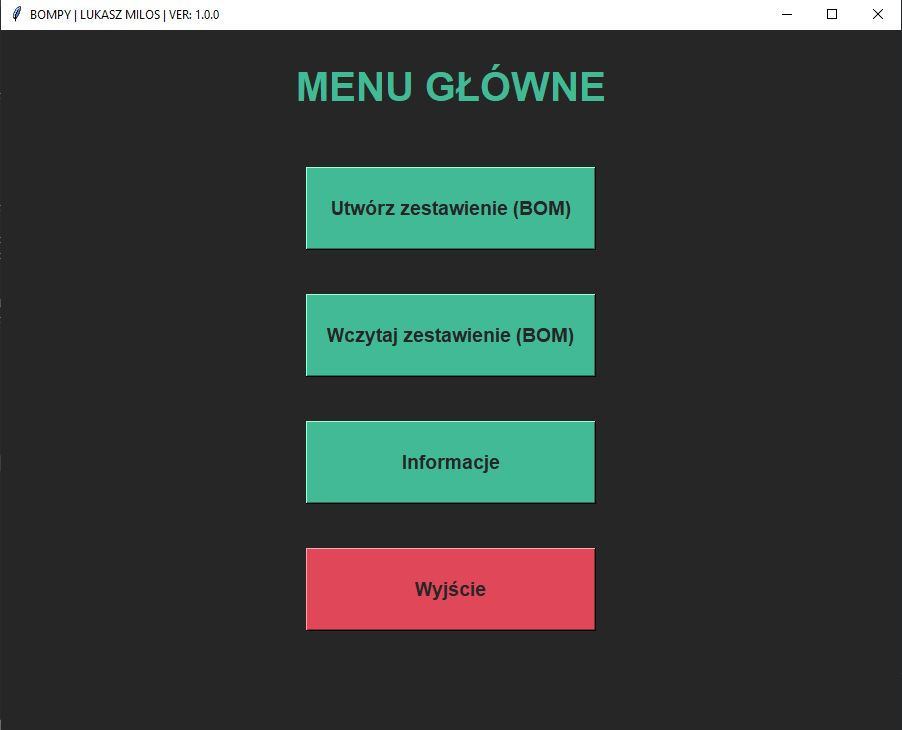
\includegraphics[width=\textwidth]{figures/app/menu.jpg}
	\caption{Menu główne aplikacji}
\label{fig:app:menu}
\end{figure}

\subsubsection*{Strona informacyjna}

Na zdjęciu (\ref{fig:app:info}) przedstawiono stronę informacyjną zawierającą krótką charakterystykę programu, autora i linki do repozytoriów.
\begin{figure}[h]
	\centering
	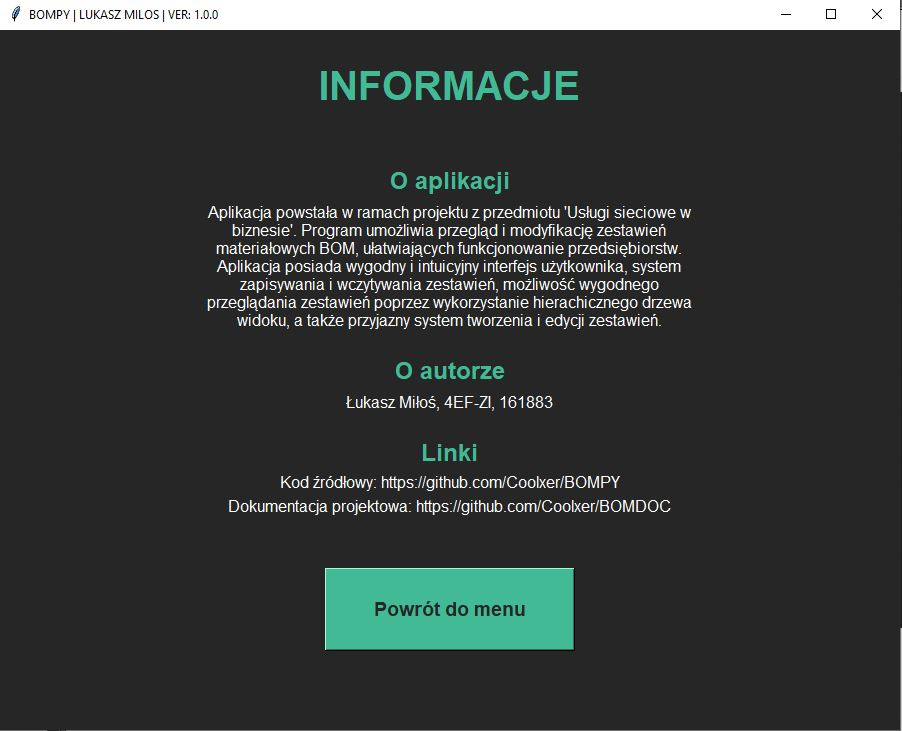
\includegraphics[width=\textwidth]{figures/app/info.jpg}
	\caption{Strona informacyjna aplikacji}
\label{fig:app:info}
\end{figure}

\subsubsection*{Wczytanie zestawienia BOM}

W kwestii wczytywania zestawienia z pliku o formacie *.json warto zwrócić uwagę na walidację poprawności pliku. Plik programowy musi być odpowiedni, tzn. przeznaczony dla tej aplikacji (odpowiedni klucz i wartość). 

W celu wczytywania pliku wykorzystano dostępne okno dialogowe (\ref{fig:app:read_file}), które odpowiednio skonfigurowano, tak aby możliwe do wyboru były jednie pliki o rozszerzeniu *.json.

\begin{figure}[h]
	\centering
	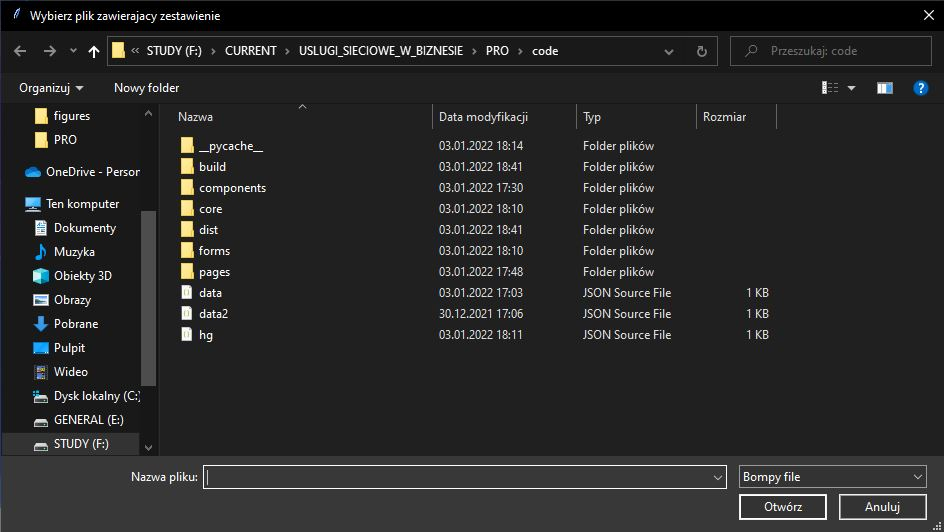
\includegraphics[width=\textwidth]{figures/app/read_file.jpg}
	\caption{Wybór pliku zestawienia}
\label{fig:app:read_file}
\end{figure}

Jeśli stwierdzona zostanie niepoprawność pliku źródłowego, zostanie wyświetlony odpowiedni komunikat (\ref{fig:app:read_file_err}).

\begin{figure}[h]
	\centering
	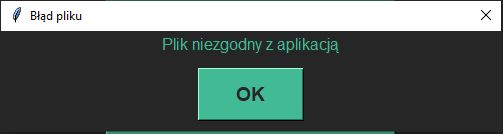
\includegraphics[width=\textwidth]{figures/app/read_file_err.jpg}
	\caption{Błędny plik zestawienia}
\label{fig:app:read_file_err}
\end{figure}


\subsubsection*{Tworzenie nowego zestawienia BOM}
Po wybraniu opcji \enquote*{Utwórz zestawienie (BOM)} z menu głównego, pojawia się okno dialogowe (\ref{fig:app:create_bom_dialog}), w którym należy podać nazwę zestawienia. 

\begin{figure}[h]
	\centering
	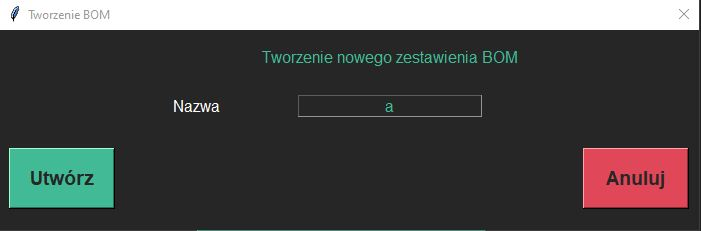
\includegraphics[width=\textwidth]{figures/app/create_bom_dialog.jpg}
	\caption{Tworzenie nowego zestawienia}
\label{fig:app:create_bom_dialog}
\end{figure}

Nazwa zestawienia musi spełniać kryterium minimum 3 znaków i maksymalnie 10 znaków. W przeciwnym razie zostanie wyświetlony stosowny komunikat (\ref{fig:app:name_too_short_err}) lub (\ref{fig:app:name_too_long_err})

\begin{figure}[h]
	\centering
	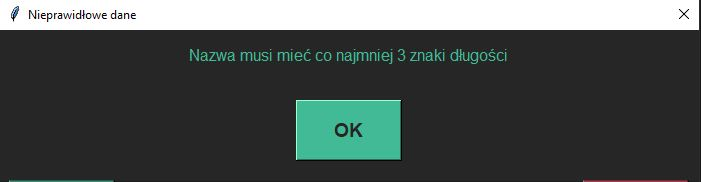
\includegraphics[width=\textwidth]{figures/app/name_too_short_err.jpg}
	\caption{Błąd zbyt krótkiej nazwy zestawienia}
\label{fig:app:name_too_short_err}
\end{figure}

\begin{figure}[H]
	\centering
	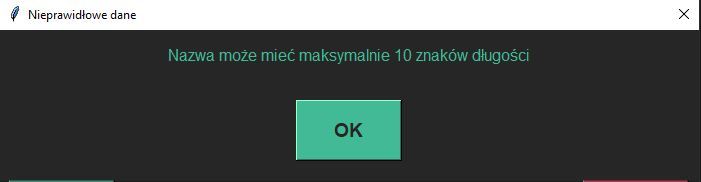
\includegraphics[width=\textwidth]{figures/app/name_too_long_err.jpg}
	\caption{Błąd zbyt długiej nazwy zestawienia}
\label{fig:app:name_too_long_err}
\end{figure}

Jeśli podana nazwa jest prawidłowa użytkownik przy użyciu stosownego okna dialogowego (\ref{fig:app:save_file}) wybiera nazwę i lokalizację pliku, w którym jego zestawienie będzie na bieżąco zapisywane.

\begin{figure}[H]
	\centering
	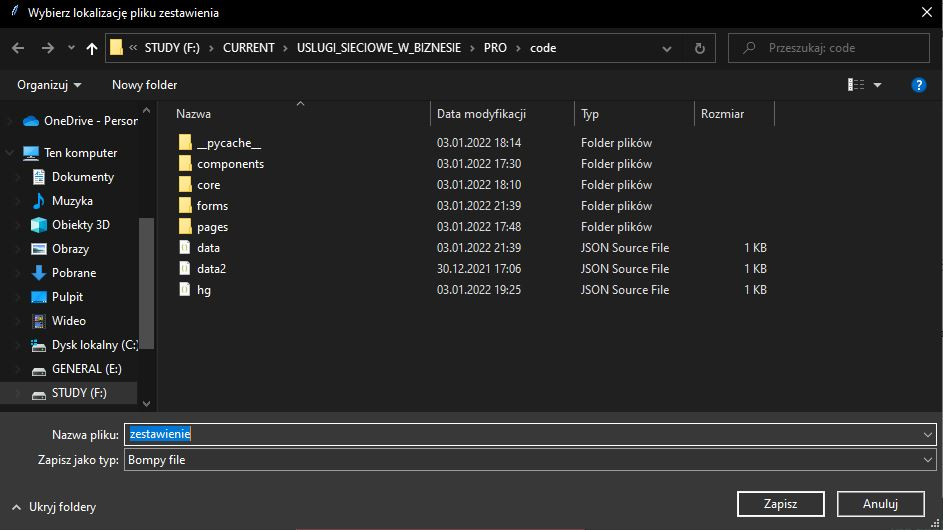
\includegraphics[width=\textwidth]{figures/app/save_file.jpg}
	\caption{Wybór nazwy i lokalizacji pliku nowego zestawienia}
\label{fig:app:save_file}
\end{figure}

\subsubsection*{Przegląd i modyfikacja zestawienia}
Po pomyślnym wczytaniu zestawienia lub utworzeniu nowego zestawienia użytkownik zostaje przekierowany na stronę prezentującą zestawienie (\ref{fig:app:bom_presentation}).

\begin{figure}[h]
	\centering
	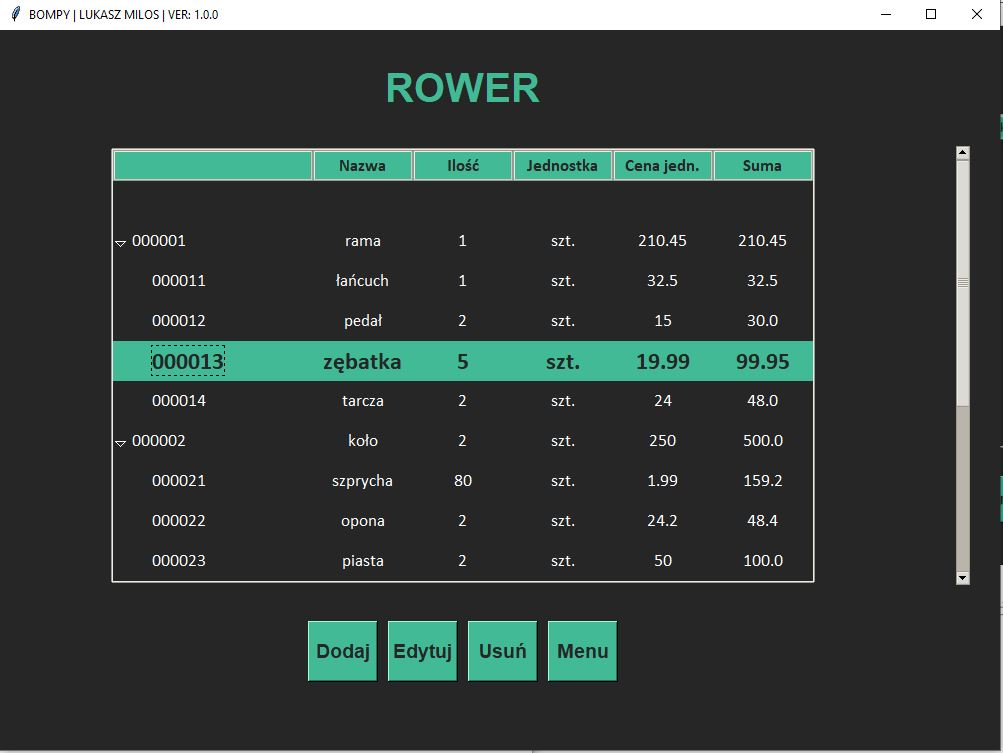
\includegraphics[width=\textwidth]{figures/app/bom_presentation.jpg}
	\caption{Prezentacja przykładowego zestawienia}
\label{fig:app:bom_presentation}
\end{figure}

Na samej górze prezentowana jest nazwa zestawienia (produktu końcowego).

Prezentowany widok drzewa składa się z 6 kolumn. Pierwsza kolumna stanowi identyfikator półproduktu, a następne oznaczają kolejno nazwę, ilość, jednostkę (kg., szt., m), cenę jednostkową i sumę (ilość * cena jednostkowa).

Widok drzewa jest strukturą hierarchiczną (możliwość zwijania i rozwijania poszczególnych wierszy). Na samej górze jest wiersz pusty, służący do dodawania komponentów składowych dla najwyższego poziomu hierarchii. Po prawej stronie widoczny jest pasek przewijania listy.

Na dole znajduje się panel sterowania, przy pomocy którego można dodać nowy komponent, edytować istniejący lub usunąć, a także powrócić do menu głównego.

Poszczególne przyciski są aktywne tylko wtedy, gdy wybrany został dowolny wiersz. Zaznaczony wiersz jest wyróżniony kolorem i powiększoną czcionką. Zaznaczenie wiersza jest konieczne nie tylko w przypadku chęci usunięcia czy edycji, ale także do dodawania nowego komponentu, ponieważ zaznaczony wiersz determinuje miejsce wstawienia nowego elementu.

\paragraph*{Dodawanie obiektu}\mbox{}\\
Na zdjęciu (\ref{fig:app:bom_add_item}) przedstawiono przykład dodawania obiektu przy użyciu specjalnie zaprojektowanego formularza. Użytkownik wypełnia poszczególne pola edycyjne. W przypadku wyboru jednostki komponentu zastosowano listę wyboru. Dla każdego interaktywnego pola tekstowego prowadzona jest walidacja poprawności (minimalna/maksymalna długość, typ tekstowy/numeryczny), a dla identyfikatora także unikatowość. W przypadku niespełnienia wymogów na ekranie wyświetlany jest stosowny komunikat modalny.

\begin{figure}[H]
	\centering
	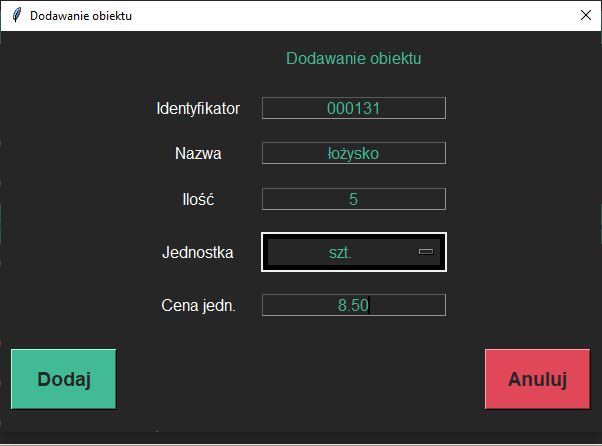
\includegraphics[width=0.7\textwidth]{figures/app/bom_add_item.jpg}
	\caption{Dodawanie obiektu}
\label{fig:app:bom_add_item}
\end{figure}

\paragraph*{Edytowanie obiektu}\mbox{}\\
Na zdjęciu (\ref{fig:app:bom_add_item}) pokazano edytowanie obiektu za pomocą formularza. Wszelkie parametry są ładowane według bieżących danych, a użytkownik może modyfikować wybrane pola. Tutaj oczywiście również jest walidacja poprawności wpisywanych danych, a także sprawdzenie integralności identyfikatora, przy czym identyfikator może pozostać niezmieniony. 

\begin{figure}[H]
	\centering
	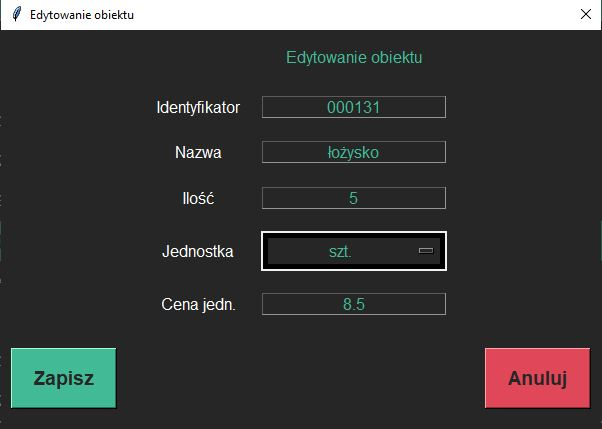
\includegraphics[width=0.7\textwidth]{figures/app/bom_edit_item.jpg}
	\caption{Edytowanie obiektu}
\label{fig:app:bom_edit_item}
\end{figure}

\paragraph*{Usuwanie obiektu}\mbox{}\\
Usuwanie wybranego obiektu przedstawiono na zdjęciu (\ref{fig:app:bom_remove_item}). Użytkownik musi potwierdzić czy żąda usunięcia danego obiektu, ponieważ zmiany są nieodwracalne.

\begin{figure}[H]
	\centering
	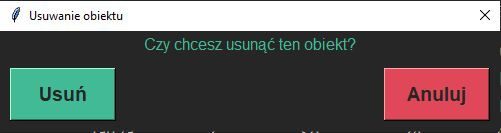
\includegraphics[width=\textwidth]{figures/app/bom_remove_item.jpg}
	\caption{Usuwanie obiektu}
\label{fig:app:bom_remove_item}
\end{figure}

Wszelkie modyfikacje (dodawanie, edytowanie, usuwanie obiektów) powodują zaktualizowanie wyświetlanej listy i automatyczny zapis nowego zestawienia do pliku.

Przy użyciu wspomnianych narzędzi użytkownik może w pełni kontrolować zestawienie materiałowe.

\clearpage
\section{Podsumowanie}
W ramach projektu stworzono pełnoprawną aplikację desktop'ową do zarządzania bazą BOM. Zagadnienie BOM (Bill Of Materials) jest istotne z perspektywy wielu przedsiębiorstw, stąd zainteresowanie tą tematyką.

Realizację tematu rozpoczęto od analizy zagadnienia i sporządzenia zaleceń programu. Następnie podjęto pewne założenia dotyczące wyboru technologii i najważniejszych kwestii programowych. 

Wybór Python'a jako języka wiodącego projektu był bardzo trafnym rozwiązaniem, ponieważ jest on bardzo intuicyjny, a wiedza i doświadczenie zdobyte podczas realizacji tego projektu z pewnością zaowocuje w przyszłości, zwłaszcza, że python rośnie w popularności i mnogości zastosowań.

Wybrana biblioteka graficzna tkinter okazała się być dość trudną w zastosowaniu, ponieważ wiele elementów należało wykonać samodzielnie. Jednak pozostałe alternatywy nie są wbudowane w interpreter i/lub wymagają płatnej licencji.

Wybór formatu *.json był oczywistą kwestią ze względu na jego hierarchiczność, a także łatwość obsługi i popularność w środowisku programistycznym.

Podczas projektowania aplikacji zadbano o modernistyczny i responsywny interfejs użytkownika, a także przejrzystość prezentowania wszelkich informacji. Dużą uwagę skupiono na estetyce kodu, wykorzystując paradygmat programowania obiektowego, a także wzbogacając kod źródłowy komentarzami.

Zdobyte w przeszłości doświadczenia spowodowały zaimplementowanie wielu walidacji danych wejściowych, a także obsługę znacznej ilości błędów.

Aplikacja umożliwia pełny przepływ informacji, rozpoczynający się od wczytania/utworzenia pliku, modyfikacji zawartości i zapisu pliku.

Esencją projektu jest wykorzystanie drzewa widoku do prezentacji zestawienia, możliwość zwijania i rozwijania poszczególnych poziomów zagnieżdżenia. Zaimplementowano także funkcje dodawania, edycji i usuwania komponentów. Do wspomnianych celów wykorzystano specjalnie zaprojektowane formularze wzbogacone o walidację danych.

W realizacji projektu wykorzystano system kontroli wersji GIT, a kod programu umieszczono na zdalnym repozytorium Github pod linkiem \url{https://github.com/Coolxer/BOMPY}.

\clearpage

\addcontentsline{toc}{section}{Źródła}
\begin{thebibliography}{5}
\bibitem{python} \url{https://docs.python.org/3/}
\bibitem{tkinter} \url{https://docs.python.org/3/library/tk.html}
\bibitem{bom_1} \url{https://www.mecalux.pl/blog/zestawienie-materialowe-bom}
\bibitem{bom_3} \url{https://www.unleashedsoftware.com/blog/everything-you-need-to-know-about-bill-of-materials}
\end{thebibliography}

\clearpage
\end{document} 
